\documentclass{article}
\usepackage[utf8]{inputenc}
\usepackage{graphicx}

\title{Rapport synthèse projet}
\author{Manon Lécubin, Aurélie Demure, Pierre Auguste, Nicolas Fernandez}
\date{October 2022}

\begin{document}

\maketitle

\section{État de l'art}

\subsection{Problématique}

Selon une étude réalisée en 2016 par ADEME et France Nature Environnement
Verdicité, 10 millions de tonnes de nourriture sont gâchées chaque
année en France. Les pertes se retrouvent à plusieurs niveaux :
\begin{itemize}
    \item la production à hauteur de 32\%
    \item la transformation des produits à hauteur de 21\%
    \item la distribution à hauteur de 14\%
    \item la consommation chez les professionnels ou les particuliers 
    pour 33\%
\end{itemize}

Nous nous sommes demandés comment réduire ce gaspillage à la source :
la production.
Celle-ci peut être réalisée par des professionels qui ont déjà des 
méthodes de récolte et des partenariats de vente mais aussi par les
particuliers. Ces derniers peuvent en effet posséder un verger et se
retrouver avec un surplus de fruits ou de légumes comparé à leur 
consommation, voire un simple manque de temps qui les empêche de les
ramasser. 

Nous nous sommes donc penchés sur les jardins des particuliers dans 
le monde rural. Selon le dictionnaire larousse, un jardin privé est un
"terrain, souvent clos, où l'on cultive des légumes, des fleurs, des 
arbres et arbustes fruitiers et d'ornement ou un mélange de ces plantes."
Le site petitsjardiniers.com ajoute que cet environnement domestique
doit être aménagé pour répondre aux besoins de la famille qui l'utilise
et à son mode de vie.

Pour cet état de l'art, nous allons donc étudier les applications ou les
démarches visant à permettre aux particuliers de vendre ou d'échanger
leurs aliments voire de les faire ramasser.

\subsection{Application SEEED}
\begin{enumerate}
    \item Idée : réseau social pour le jardin : mise en contact de
    cultivateurs et particuliers pour faire du troc. Possibilité 
    d'échanger par messages et de vendre ses produits.
    \item Fonctionnement : inscription ou connexion via Facebook et
    personnalisation du profil avec le nom et une photo.
    Utilisation de la localisation et calcul d'une distance autour
    pour présenter des jardins proches (disponibles sous forme de carte).
    Profil acheteur qui peut repérer les offres environantes.
    Profil cultivateur qui vend ou propose un troc.
    Les deux ne sont pas incompatibles.
    Mise en place d'une messagerie pour échanger et finaliser les affaires.
    \item Historique : budget de départ pour l'application : 5000€
    
    Très récente : départ du développement début 2021.
    \item Analyse : application novatrice avec un objectif éthique,
    cependant peu de recul sur la fiabilité de la plateforme notamment
    au niveau de l'utilisation et de la gestion des données avec Facebook.
\end{enumerate}
https://seeed-app.fr/ 

\subsection{Application et site LePotiron} 
\begin{enumerate}
    \item Idée : trocs, dons, ventes de surplus et rencontres car on produit
    souvent plus que ce qu'on peut ou veut consommer.
    \item Fonctionnement : site gratuit où l'on :
    \begin{itemize}
        \item renseigne une ville
        \item choisit des produits parmi ceux disponibles dans notre entourage
        \item remplit un formulaire de mise en contact
    \end{itemize}
        \item Historique : présentée à la première édition française du startupweekend à Paris. Elle existe depuis 2010 mais s'est 
    renouvelé récemment (2017) en raison d'une ancienne équipe indisponible et de problèmes
    techniques liés à l'inscription.
    \item Analyse : premier site de mise en relation des particuliers et petits producteurs sur une base de produits locaux. Il trouve sa raison d'être dans les engagements écologiques des français.
    Mise en place d'un blog (https://www.lepotiblog.com/) dans la continuité
    de leurs valeurs écologiques et humaines.
\end{enumerate}
https://www.lepotiron.fr/
\subsection{PlantCatching} Plateforme ayant existé une dizaine d'années mais
qui a dû fermer le 6 octobre 2022 du fait de la concurrence de Facebook
(plus assez d'utilisateurs). A la différence des deux précédentes, elle
permettait également le partage de graines, de plantes et de matériaux de
jardinage.

\subsection{Site Fruiteefy}
\begin{enumerate}
    \item Idée : créer un réseau pour produire et consommer autrement
    avec une carte interactive et des recherches par ville.
    \item Fonctionnement : créer un compte et donner des informations sur
    son jardin si l'on en possède un pour accéder aux ventes de proximité. 
    \item Analyse : s'inscrit dans une dynamique nationale de valorisation
    des circuits courts et de la consommation locale rémunérant les
    producteurs (qui acquiert une certaine visibilité). Est soutenue par
    plusieurs organismes tels que la région Occitanie et la communauté du 
    Coq Vert qui résulte d'un partenariat entre le Ministère de la 
    Transition Ecologique et ADEME.
\end{enumerate}
https://www.fruiteefy.fr/
https://www.bpifrance.fr/nos-actualites/communaute-du-coq-vert-un-engagement-pour-le-climat

\subsection{Leaf}
\begin{enumerate}
    \item Idée : localiser et acheter des produits frais entre particuliers.
    Solution économique pour les vendeurs et consommation saine pour les
    acheteurs.
    \item Fonctionnement : application gratuite qui permet d'accéder à
    des produits de tout le terroir français. aucun frais sur les
    transactions.
    \item Historique : cette application est née grâce à une fille 
    d'agriculteurs qui ne trouvait pas comment s'approvisionner en 
    produits frais sans devoir retourner chez ses parents.
    S'inscrit aujourd'hui dans le Plan Alimentaire Territorial.
    \item Analyse : les petits producteurs ne sont pas inclus dans le 
    programme et la consommation locale n'est pas valorisée.
\end{enumerate}
https://www.leafapp.fr/

\subsection{Initiative Aux Arbres Citoyens}
\begin{enumerate}
    \item Idée : effectuer des cueillettes collectives et solidaires
    chez des propriétaires d'arbres fruitiers pour les redistribuer
    aux plus démunis.
    \item Fonctionnement : les bénévoles et propriétaires peuvent récupérer
    ce qu'ils souhaitent de la récolte mais dans les faits les dons sont
    de l'ordre de 80\%.
    \item Historique : fondée en juillet 2020 à la Rochelle sur trois
    valeurs: la lutte contre le gaspillage
             - les circuits courts
             - la solidarité
    \item Analyse : initiative contre le gaspillage qui est réalisée par
    des bénévoles mais ne s'insert dans aucune application.
\end{enumerate}

\subsection{Conclusion}

Des applications réussissent déjà à mettre en lien des particuliers pour
le troc ou la vente de fruits et légumes. La plupart sont florissantes même 
si la concurrence semble importante.

Cependant aucune de ces applications ne semblent proposer un équivalent à l'initiative Aux Arbres Citoyens.


De plus les invendus de l'application pourraient être proposés à des 
associations à l'approche de leur date de péremption.


Nous allons donc chercher à insérer ces deux idées dans notre application
pour proposer aux consommateurs et producteurs un modèle plus complet.

\vspace{8mm}

\section{Cahier des charges}

\subsection{Contexte et description du projet}

Les pommes, c'est bon. C'est encore mieux quand elles viennent de notre jardin. On sait comment elles ont été faites, elles sont bios, locales, et c'est ce qui nous les fait aimer encore plus. Mais quand notre pommier est trop gros, on a trop de pommes, et bien souvent la majorité tombent par terre et ne sont jamais récupérées. De même quand on part en voyage et qu'on ne peut pas les ramasser, elles pourrissent aussi sans qu'on puisse en profiter.

Mais pourquoi ne pas en faire profiter les autres ? Comment trouver un moyen d'avertir les personnes intéressées de notre surplus de fruits ou légumes ? C'est de là que vient l'idée de notre application web : une interface de rencontre et de partage, pour échanger, donner et recevoir des fruits et légumes locaux, et venir en aide à nos voisins.
Facilitant l'accès à des produits bios et locaux, cette application permet aux personnes de vendre ou donner ce qu'ils ont cultivé, ou de rechercher des produits près de chez eux. Pour cela rien de plus simple ; il suffit de s'inscrire, renseigner sa localisation, et spécifier nos besoins. Grâce à une carte interactive, on peut facilement avoir accès à ce que proposent nos voisins.

Envie de vendre, échanger ou donner ses produits ? Besoin d'aide pour les récoltes que l'on ne peut pas effectuer ? Une petite annonce et le tour est joué ! Et en y ajoutant des photos, les autres utilisateurs se feront une meilleure idée. Mais si personne ne veut de mes produits ? Pas de panique, si au bout d'un certain temps personne ne se propose, l'application vous donnera la possibilité de faire don à une association.
Une envie de fruits ou légumes en particulier ? Vous pouvez simplement faire une recherche, et l'application vous retourne les résultats près de chez vous. Quelque soit votre besoin, les propositions tiendront compte de la distance géographique.
Enfin, lorsque vous trouvez des personnes intéressées, un système de messagerie permet alors d'échanger diverses informations, de discuter, et d'avoir une trace des engagements de chacun.

Ainsi, cette application web permet aux jardins privés de limiter le gaspillage, mais aussi d'échanger avec d'autres personnes qui partagent vos envies.

\subsection{Objectif et périmètre du projet}

Nous souhaitons ainsi offrir à nos utilisateurs un service plus complet que ceux existant actuellement. Une application qui leur permet de gérer leurs surplus, mais également d'aider à la récolte même, un élément souvent oublié lorsque l'on parle de gaspillage.
Pour cela, nous nous concentrerons sur tout le territoire français.

Notre projet consiste en une application web permettant de vendre et d'échanger ses fruits et légumes, tout en proposant des cueillettes directement chez le particulier. Pour cela, il y aura possibilité de déposer des annonces de vente de fruits et légumes, de troc ou encore de cueillette. 

Chaque particulier pourra alors rechercher le produit qu'il désire parmi ces annonces proches de chez lui. En effet, une carte interactive permettra de voir la localisation des différents produits, cette localisation ne sera pas précise mais donnée par zone géographique. Les produits seront proposés dans un périmètre donné autour de la localisation du client, périmètre qui augmentera au fil du temps, dans un objectif de limiter la consommation de carburant provoquée par de longs trajets et donc la pollution atmosphérique. 

Un système de messagerie permettra de mettre en contact la personne intéressée et la personne proposant le produit, afin qu'elles puissent convenir d'une date et d'un lieu de rendez-vous. 
La problématique des cambriolages s'est posée lors de la réflexion sur le système de cueillette, cependant chaque particulier ne donnera sa localisation précise uniquement s'il le souhaite via la messagerie et décidera seul s'il accepte qu'une autre personne vienne chez lui sans sa présence. De plus, les cueillettes peuvent également se faire lorsque la personne est présente, par exemple lors d'une journéé de télé-travail.

Dans les derniers jours de consommation du produit, s'il n'a pas pu être vendu ou échangé, il sera proposé à l'utilisateur d'en faire don à une association. 


\subsection{Description fonctionnelle des besoins}

\begin{tabular}{|p{3.5cm}|p {3.5cm}|c|c|c|} \hline
    Fonction & Objectif & Degré de liberté & Niveau de priorité  \\ \hline
    Permettre à l'utilisateur de proposer ses fruits  & Saisir facilement ses informations & Faible & Élevé \\ \hline
    Accéder à l'ensemble des informations via une carte interactive & Permettre à l'utilisateur de s'y retrouver facilement & Moyen & Moyen \\ \hline
    Permettre aux utilisateurs de se contacter via l'application & Faciliter les échanges entre utilisateurs & Élevé & Moyen \\ \hline
    Renvoyer vers une association & Ne pas gaspiller alors que des solutions existent & Faible & Élevé \\ \hline
\end{tabular}


\subsection{Enveloppe budgétaire et ressources disponibles}

Ce projet n'a pas de budget alloué. L'équipe projet est composée de 4 membres qui travailleront directement avec leurs matériels personnels ou celui de l'établissement.

\subsection{Délais}

Le projet se décompose en différents livrables et différentes échéances:
\begin{itemize}
    \item Le premier livrable se compose d'un rapport à déposer avant le 20/10/2022.
    \item Le second livrable correspond au rendu du projet. Ce dernier a lieu le 06/01/2023.
\end{itemize}

\vspace{8 mm}


\section{Charte Projet}

\subsection{Contexte}

Aujourd'hui, les circuits courts sont les alternatives les plus intéressantes face au défi qu'est devenu la gestion de l'alimentation et de l'eau. De nombreuses solutions sont apparues pour faire face à ce défi. On peut retrouver les jardins partagés, les micro-fermes mais également le partage de ressources produites au sein de jardins privés. 

Ces applications sont principalement utilisées par les propriétaires de jardin privés. Chacune d'entre elles permet de répondre à sa manière à la problématique du surplus de production dans ces jardins ainsi que leur gestion.

Le cahier des charges permet d'identifier de manière immédiate les principaux besoins et fonctions auxquels l'application doit répondre. Il s'agit notamment de permettre de mettre en relation des propriétaires de jardins privés, de permettre de gérer le surplus de production mais également de permettre une meilleure gestion de la récolte afin d'éviter les pertes initiales.


\subsection{Finalités et importance du projet: Business Case}

Ce projet est aujourd'hui essentiel afin de répondre aux problématiques actuelles concernant la gestion de l'alimentation en circuits courts. De plus, la nature même du projet et ses coûts extrêmements limités réduisent la néceesité d'un retour sur investissement, permettant ainsi un départ peu risqué. L'application visant à proposer un service sans recherche de bénéfices, l'estimation de ces derniers est inutile.

De manière prévisionnelle, on peut estimer que l'application permettra de mettre en relation de nombreux propriétaires de jardins privés au sein de communes principalement en zone rurale. Sa gestion des récoltes participera à une nouvelle manière de partager des surplus de fruits non consommés, une innovation qui permettra une ouverture plus grande que la plupart des projets existants.

\vspace{4mm}

Les parties prenantes relatives au projets sont: l'équipe projet, composée de quatre membres, les enseignants encadrants, ainsi que les potentiels utilisateurs de l'application.

Le périmètre du projet s'étend sur tout le territoire français, mais la nature même de son fonctionnement favorise une utilisation dans des zones rurales où le nombre de jardins privés est bien plus important.
A cette limite géographique s'ajoutent de nombreux prérequis à obtenir: obtention des compétences nécessaires au développement d'une application web et de la création d'algorithme, être dans un cadre légal quant à la possibilité de venir récolter les fruits chez une autre personne.

\vspace{4mm}
 
Cette analyse du Business Case permet de proposer une matrice SWOT identifiant les forces, faiblesses, opportunités ainsi que menaces du projet.

\vspace{2mm}             
  
\begin{centering}
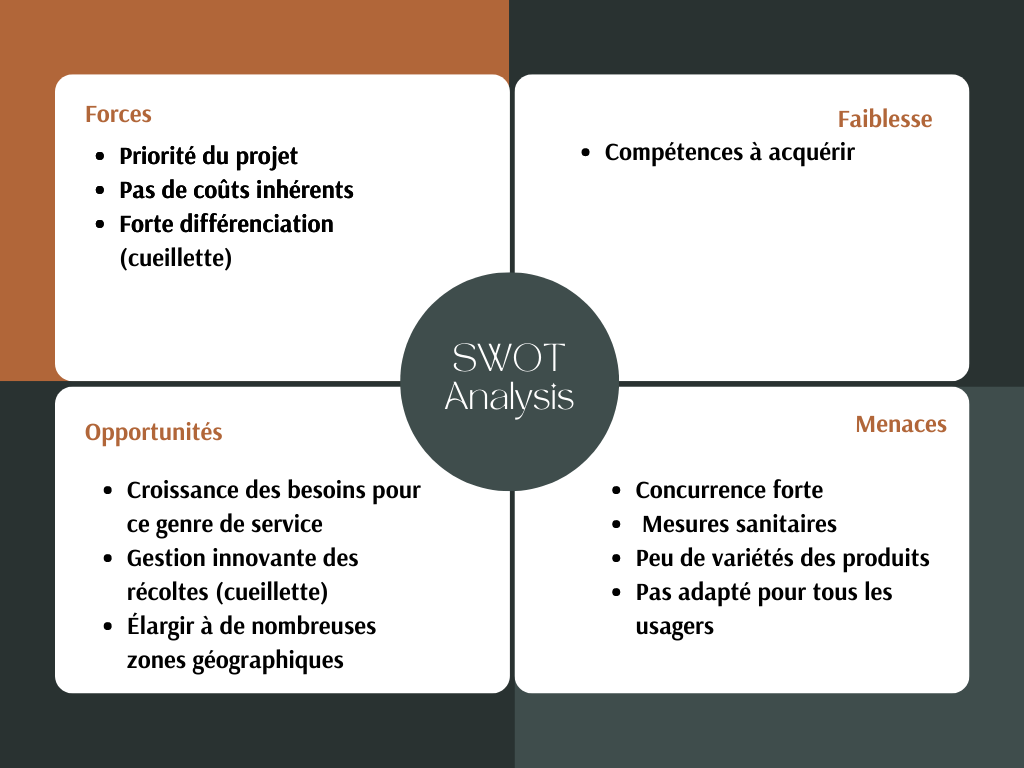
\includegraphics[width = 12cm, height = 9 cm]{SWOTF.png}
\end{centering}

\maketitle
\subsection{Objectifs et résultats opérationnels}

Ces applications connaissent un franc succès aujourd'hui, de par la nécessité de faire face au défi du gaspillage alimentaire, ainsi que par le développement des circuits courts. L'innovation ici proposée, concernant la participation à la récolte même des fruits, permet de s'attaquer à l'une des principales causes de perte de ces derniers. Ces différents éléments sont des indicateurs de la possibilité de succès de ce projet.

\subsection{Ressources}
Les moyens à mobiliser sont :
PC personnels et/ou de l'école, postgress4SQL, python3 


\subsection{Jalons}
\begin{center}
\begin{tabular}{|p{3cm}|p{5cm}|p{2cm}|} 
  \hline
  Jalon & Description & Date \\
  \hline
  Etape 1 : Exigences opérationnelles & Validation de l'idée lors de la soutenance & 22/10/22 \\
  \hline
  Etape 2 : Création de la base de données & Création de la base de données relative aux fruits et légumes disponibles &  \\
  \hline
  Etape 3 : Réalisation de l'interface & Réalisation de l'interface utilisateur & \\
  \hline
  Etape 4 : Réalisation messagerie & 
  Réalisation d'un système de contact entre les utilsateurs (messagerie) pour obtenir plus d'informations sur un produit en vente ou les conditions d'accueil pour une cueillette & \\
  \hline
  Etape 5 : Ajout d'une carte & Ajout d'une carte permettant de repérer où se situent les fruits et légumes & \\
  \hline
  Etape 6 : Ajout de restrictions sur la carte & Ajouter des rayons sur la carte par rapport à la localisation du client, qui augmentent au cours du temps & \\
  \hline
  Etape 7 : Ajout d'une fonctionnalité pour les dons & Ajouter une fonction qui permet au client de donner ses produits dans les derniers jours de consommation possibles du produit & \\ 
  \hline
\end{tabular}
\end{center}


\subsection{Risques/Opportunités}

Risques : applications utilisant le même concept déjà établies sur le marché.


Opportunités : le système de cueillette directement chez le particulier n'a pas encore été utilisé et permettrait de fortement réduire le gâchis

\end{document}
